%iffalse
\let\negmedspace\undefined
\let\negthickspace\undefined
\documentclass[journal,12pt,onecolumn]{IEEEtran}
\usepackage{cite}
\usepackage{amsmath,amssymb,amsfonts,amsthm}
\usepackage{algorithmic}
\usepackage{graphicx}
\usepackage{textcomp}
\usepackage{xcolor}
\usepackage{txfonts}
\usepackage{listings}
\usepackage{enumitem}
\usepackage{mathtools}
\usepackage{gensymb}
\usepackage{comment}
\usepackage[breaklinks=true]{hyperref}
\usepackage{tkz-euclide} 
\usepackage{listings}

\usepackage{booktabs}
\usepackage{pgfplots}
\usepackage{gvv}                                        
\usepackage[latin1]{inputenc}     
\usepackage{xparse}
\usepackage{color}                                            
\usepackage{array}                                            
\usepackage{longtable}                                       
\usepackage{calc}                                             
\usepackage{multirow}
\usepackage{multicol}
\usepackage{hhline}                                           
\usepackage{ifthen}                                           
\usepackage{lscape}
\usepackage{tabularx}
\usepackage{array}
\usetikzlibrary{patterns}
\usepackage{siunitx}
\pagestyle{empty}
\usetikzlibrary{calc}
\usepackage[margin=1in]{geometry}
\usepackage{pgffor}
\usepackage{float}
\usepackage{pgf-pie}
\newtheorem{theorem}{Theorem}[section]
\newtheorem{problem}{Problem}
\newtheorem{proposition}{Proposition}[section]
\newtheorem{lemma}{Lemma}[section]
\newtheorem{corollary}[theorem]{Corollary}
\newtheorem{example}{Example}[section]
\newtheorem{definition}[problem]{Definition}
\newcommand{\BEQA}{\begin{eqnarray}}
\newcommand{\EEQA}{\end{eqnarray}}
\newcommand{\define}{\stackrel{\triangle}{=}}
\theoremstyle{remark}
\newtheorem{rem}{Remark}
% Marks the beginning of the document
\pgfplotsset{compat=1.18}
\begin{document}

\bibliographystyle{IEEEtran}
\vspace{3cm}

\title{2024-ST-'53-65'}
\author{EE24BTECH11023}
%\maketitle
%\newpage
%\bigskip
\maketitle

{\let\newpage\relax\maketitle}

\renewcommand{\thefigure}{\theenumi}
\renewcommand{\thetable}{\theenumi}
\setlength{\intextsep}{10pt} % Space between text and floats

\numberwithin{equation}{enumi}
\numberwithin{figure}{enumi}
\renewcommand{\thetable}{\theenumi}



\begin{enumerate}
    \item Which one of the following statements is TRUE about the continuity equation $$\frac{\partial u}{\partial x}+\frac{\partial u}{\partial y}+\frac{\partial u}{\partial z}$$
 (where $u$, $v$, $w$ are the velocity components along the $x$, $y$, and $z$ coordinates, respectively):
    \begin{enumerate}
        \item The equation is valid only for steady incompressible flows.
        \item The equation is valid for both steady and unsteady incompressible flows.
        \item The equation is valid only for steady compressible flows.
        \item The equation is valid only for unsteady compressible flows.
    \end{enumerate}

    \item The head loss $(K_L)$ associated with the flow entry of water to an internal passage depends on the shape of the entry. The following figure shows three different types of flow entry into a pipe. Which one of the following relationships correctly represents the head loss associated with the three different flow entries?
    \begin{figure}[H]
        \centering
         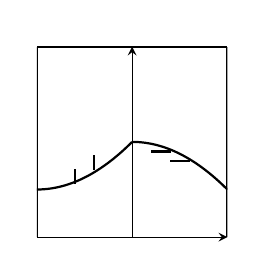
\begin{tikzpicture}
        \begin{axis}[
            axis lines = middle,
            xlabel = $ $,
            ylabel = $ $,
            xmin = -0.5, xmax = 0.5,
            ymin = 0, ymax = 1,
            xtick = {0},
            ytick = {0},
            x label style={at={(axis description cs:1,0)},anchor=west},
            y label style={at={(axis description cs:0,1)},anchor=south},
            extra tick style={grid=major},
            width=4cm, height=4cm,
            samples=100,
            domain=-0.5:0.5,
        ]
                \addplot[domain=-0.5:0, samples=100, thick] {0.25+(x+0.5)^2};
                \draw [thick](-0.5,0) -- (-0.5,1);
                \draw [thick](0.5,0) -- (0.5,1);
                \draw [thick](0.5,1) -- (-0.5,1);
                \addplot[domain=0.1:0.2, samples=100, thick] {0.45};
                \addplot[domain=0.2:0.3, samples=100, thick] {0.40};
                \draw [thick](-0.2,0.35) -- (-0.2,0.43);
                \draw [thick](-0.3,0.28) -- (-0.3,0.36);
        \addplot[domain=0:0.5, samples=100, thick] {0.5-x^2};
        \end{axis}
    \end{tikzpicture}
    
  
    \end{figure}
    \begin{enumerate}
        \item $(K_L)_a > (K_L)_b > (K_L)_c$
        \item $(K_L)_b > (K_L)_a > (K_L)_c$
        \item $(K_L)_b \leq (K_L)_a = (K_L)_c$
        \item $(K_L)_b < (K_L)_a < (K_L)_c$
    \end{enumerate}

    \item The form and friction drags together contribute to the total drag when flow of air occurs past any object. Two orientations of a finite flat plate are shown in the figure. In Orientation-1, the plate is placed perpendicular to the flow, while in Orientation-2, the plate is placed parallel to the flow. If the velocity $(V)$ of air in both orientations is the same, which one of the following options is TRUE?
    \begin{figure}[H]
        \centering
        \begin{center}
    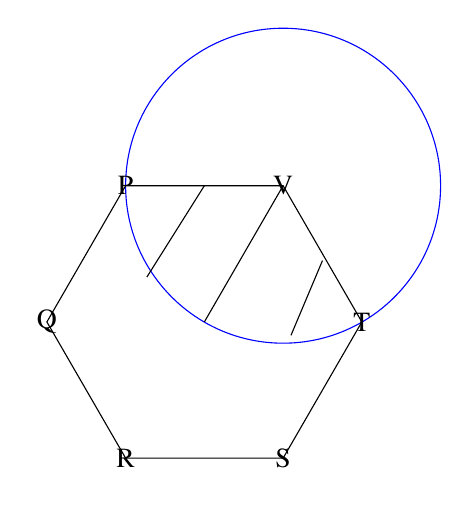
\begin{tikzpicture}
            \draw[blue] (2,3.46) circle (2);
            \draw(1,3.46)--(0.27,2.3);
            \draw(2,3.46)--(1,1.73);
            \draw(2.5,2.509)--(2.1,1.56);
        \draw (0,0) -- (2,0) -- (3,1.73) -- (2,3.46) -- (0,3.46) -- (-1,1.73) -- cycle;
        \node at (0,0) {R};
        \node at (2,0) {S};
        \node at (3,1.73) {T};
        \node at (2,3.46) {V};
        \node at (0,3.46) {P};
        \node at (-1,1.73) {Q};
    \end{tikzpicture}
    \end{center}  
    \end{figure}
    \begin{enumerate}
        \item Orientation-1 has higher form drag and lower friction drag, and Orientation-2 has lower form drag and higher friction drag.
        \item Orientation-1 has lower form drag and lower friction drag, and Orientation-2 has higher form drag and higher friction drag.
        \item Orientation-1 has lower form drag and higher friction drag, and Orientation-2 has higher form drag and lower friction drag.
        \item Orientation-1 has higher form drag and higher friction drag, and Orientation-2 has lower form drag and lower friction drag.
    \end{enumerate}

    \item A spherical ball is steadily supported against gravity by an upward air jet. Take acceleration due to gravity to be $g = 10 \, \text{m/s}^2$. The mass flow rate of air, reaching the ball, is $0.01 \, \text{kg/s}$, and the air reaches the ball at an upward velocity of $3 \, \text{m/s}$. Neglecting the buoyancy force, and using the principle of integral momentum balance, the mass (in grams, up to one decimal place) of the ball is {\underline{\hspace{2cm}}}.
    \begin{figure}[H]
        \centering
        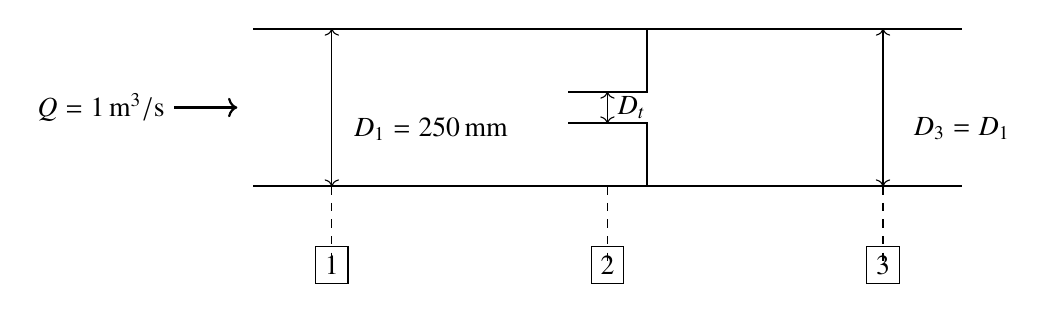
\begin{tikzpicture}
    \draw[thick] (-1, 1) -- (8, 1); 
    \draw[thick] (-1, -1) -- (8, -1); 
    \draw[->, thick] (-2, 0) -- (-1.2, 0);
    \node[left] at (-2, 0) {$Q = 1 \, \mathrm{m^3/s}$};
    \draw[<->] (0, 1) -- (0, -1);
    \node[below] at (1.256, 0) {$D_1 = 250 \, \mathrm{mm}$};
    \draw[thick] (4, -1) --(4, -0.2)--(3,-0.2);
    \draw[thick](4, 1) --(4, 0.2)--(3,0.2);  
    \draw[<->] (3.5, 0.2) -- (3.5, -0.2);
    \node[right] at (3.5, 0) {$D_t$};
    \draw[<->] (7, 1) -- (7, -1);
    \node[below] at (8, 0) {$D_3 = D_1$};
    \node[draw, rectangle] at (0, -2) {1};
    \draw[dashed] (0, -1) -- (0, -2);
    \node[draw, rectangle] at (3.5, -2) {2};
    \draw[dashed] (3.5, -1) -- (3.5, -2);
    \node[draw, rectangle] at (7, -2) {3};
    \draw[dashed] (7, -1) -- (7, -2);
\end{tikzpicture}

  
    \end{figure}

    \item The incompressible flow of air over a curved surface having possible flow separation is schematically shown in the figure. Two zones P and Q are indicated in the figure. Which one of the following combinations is TRUE for zones P and Q?
    \begin{figure}[H]
        \centering
        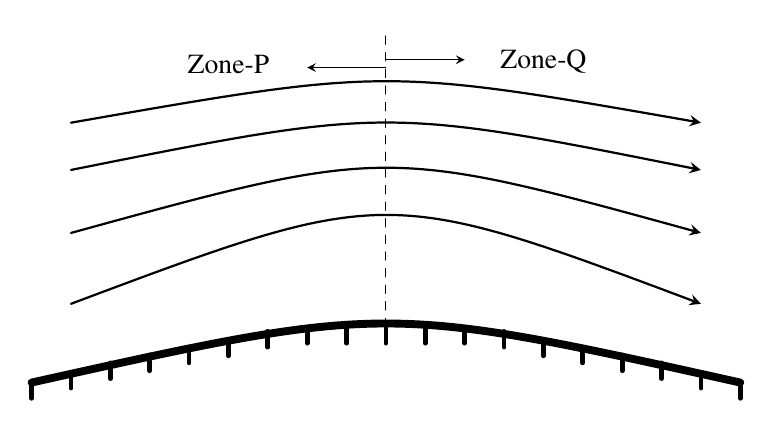
\begin{tikzpicture}[line cap=round, line join=round, >=stealth]
    \draw[line width=1mm] (-4.5,-1) .. controls (0,0) .. (4.5,-1); 
    \draw[->, thick] (-4,2.3) .. controls (0,3) .. (4,2.3);
    \draw[->, thick] (-4,1.7) .. controls (0,2.5) .. (4,1.7);
    \draw[->, thick] (-4,0.9) .. controls (0,2) .. (4,0.9);
    \draw[->, thick] (-4,0) .. controls (0,1.5) .. (4,0); 
    \draw[dashed] (0,-0.5) -- (0,3.5);
    \node[above] at (-2,2.8) {Zone-P};
    \node[above] at (2,2.8) {Zone-Q};
    \draw[->](0,3)--(-1,3);
    \draw[->](0,3.1)--(1,3.1);

    \draw[line width=0.6mm] (0,-0.3)--(0,-0.5);
    \draw[line width=0.6mm] (0.5,-0.3)--(0.5,-0.5);
    \draw[line width=0.6mm] (1,-0.3)--(1,-0.5);
    \draw[line width=0.6mm] (1.5,-0.35)--(1.5,-0.55);
    \draw[line width=0.6mm] (2,-0.46)--(2,-0.66);
    \draw[line width=0.6mm] (2.5,-0.55)--(2.5,-0.75);
    \draw[line width=0.6mm] (3,-0.65)--(3,-0.85);
    \draw[line width=0.6mm] (3.5,-0.75)--(3.5,-0.95);
    \draw[line width=0.6mm] (4,-0.87)--(4,-1.07);
    \draw[line width=0.6mm] (4.5,-1)--(4.5,-1.2);

    \draw[line width=0.6mm] (-0.5,-0.3)--(-0.5,-0.5);
    \draw[line width=0.6mm] (-1,-0.3)--(-1,-0.5);
    \draw[line width=0.6mm] (-1.5,-0.35)--(-1.5,-0.55);
    \draw[line width=0.6mm] (-2,-0.46)--(-2,-0.66);
    \draw[line width=0.6mm] (-2.5,-0.55)--(-2.5,-0.75);
    \draw[line width=0.6mm] (-3,-0.65)--(-3,-0.85);
    \draw[line width=0.6mm] (-3.5,-0.75)--(-3.5,-0.95);
    \draw[line width=0.6mm] (-4,-0.87)--(-4,-1.07);
    \draw[line width=0.6mm] (-4.5,-1)--(-4.5,-1.2);


\end{tikzpicture}
  
    \end{figure}
    (a) Acceleration of flow,(b) Deceleration of flow,(c) Adverse pressure gradient,(d)Favorable pressure gradient,(e) No flow separation (f) Possible flow seperation.
    \begin{enumerate}
        
        \item \underline{P: (a), (d), (e)} and \underline{Q: (b), (c), (f)}
        \item \underline{P: (a), (c), (e)} and \underline{Q: (a), (d), (e)}
        \item \underline{P: (a), (d), (f)} and \underline{Q: (b), (d), (e)}
        \item \underline{P: (a), (c), (e)} and \underline{Q: (a), (f), (e)}
            \end{enumerate}

    \item A spherical metal ball (of density $\rho_s$ and diameter $D$), attached to a string, is exposed to a crossflow (of velocity $U_{\infty}$) of a viscous fluid (of viscosity $\mu$ and density $\rho_f$). Due to the crossflow, the string makes an angle of inclination, $\theta$, with the top surface as shown in the figure. The acceleration due to gravity is denoted by $g$. For this flow, Reynolds number, $\text{Re}=\frac{{\rho_f}U_{\infty}D}{\mu} \ll 1$ and buoyancy force in the fluid is negligible compared to viscous force. Assuming the string to be weightless and offering negligible drag, derive the expression for $\theta$ is 
    \begin{figure}[H]
        \centering
        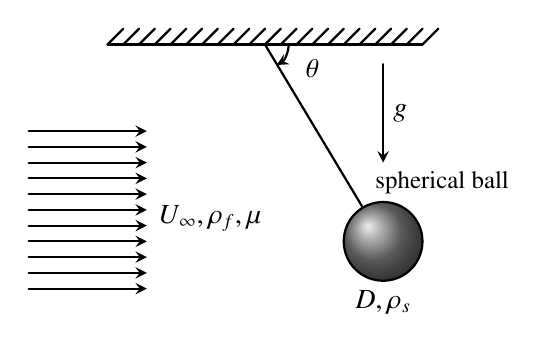
\begin{tikzpicture}[line cap=round, line join=round, >=stealth]
    \draw[thick] (-2,0) -- (2,0);
    \draw[thick] (0,0) -- (1.5,-2.5);
    \shade[ball color=gray] (1.5,-2.5) circle (0.5);
    \draw[thick] (1.5,-2.5) circle (0.5);
    \draw[->, thick] (1.5,-0.25) -- (1.5,-1.5) node[midway,right] {$g$};
    \draw[->, thick] (-3,-2.5) -- (-1.5,-2.5);
    \draw[->, thick] (-3,-2.3) -- (-1.5,-2.3);
    \draw[->, thick] (-3,-2.7) -- (-1.5,-2.7);
    \draw[->, thick] (-3,-2.9) -- (-1.5,-2.9);
    \draw[->, thick] (-3,-2.1) -- (-1.5,-2.1);
    \draw[->, thick] (-3,-1.9) -- (-1.5,-1.9);
    \draw[->, thick] (-3,-1.7) -- (-1.5,-1.7);
    \draw[->, thick] (-3,-3.1) -- (-1.5,-3.1);
    \draw[->, thick] (-3,-1.5) -- (-1.5,-1.5);
    \draw[->, thick] (-3,-1.3) -- (-1.5,-1.3);
    \draw[->, thick] (-3,-1.1) -- (-1.5,-1.1);
    \node[below] at (1.5,-3) {$D, \rho_s$};
    \node[above] at (-0.7,-2.5) {$U_{\infty},\rho_f,\mu$};
    \node at (2.25,-1.75) {\small spherical ball};
    \draw[thick,->] (0.3,0) arc[start angle=0, end angle=-60, radius=0.3];
    \node at (0.6,-0.3) {$\theta$};
    \draw[thick](-2,0)--(-1.8,0.2);
    \draw[thick](-1.8,0)--(-1.6,0.2);
    \draw[thick](-1.6,0)--(-1.4,0.2);
    \draw[thick](-1.4,0)--(-1.2,0.2);
    \draw[thick](-1.2,0)--(-1,0.2);
    \draw[thick](-1,0)--(-0.8,0.2);
    \draw[thick](-0.8,0)--(-0.6,0.2);
    \draw[thick](-0.6,0)--(-0.4,0.2);
    \draw[thick](-0.4,0)--(-0.2,0.2);
    \draw[thick](-0.2,0)--(0,0.2);
    \draw[thick](0,0)--(0.2,0.2);
    \draw[thick](0.2,0)--(0.4,0.2);
    \draw[thick](2,0)--(2.2,0.2);
    \draw[thick](1.8,0)--(2,0.2);
    \draw[thick](1.6,0)--(1.8,0.2);
    \draw[thick](1.4,0)--(1.6,0.2);
    \draw[thick](1.2,0)--(1.4,0.2);
    \draw[thick](1,0)--(1.2,0.2);
    \draw[thick](0.8,0)--(1,0.2);
    \draw[thick](0.6,0)--(0.8,0.2);
    \draw[thick](0.4,0)--(0.6,0.2);
    
\end{tikzpicture}
  
    \end{figure}
    \begin{enumerate}
        \item $\tan^{-1}({\frac{1}{18}}{\frac{D^2{\rho_s}^2{g}}{U_{\infty} \mu \rho_f}}) $
        \item $\tan^{-1}({\frac{1}{18}}{\frac{D^2{\rho_f}{g}}{U_{\infty} \mu}})$
        \item $\tan^{-1}({\frac{2}{9}}{\frac{D^2{\rho_s}{g}}{U_{\infty} \mu}})$
        \item $\tan^{-1}({\frac{1}{18}}{\frac{D^2{\rho_s}{g}}{U_{\infty} \mu}})$
    \end{enumerate}

    \item In a Cartesian coordinate system, a steady, incompressible velocity field of a Newtonian fluid is given by 
    $$\vec{V} = u_0(1 - ay^2) \, \hat{i}$$
    Here, $V$ is the velocity vector in $m/s$, i is the unit vector in the x-direction,$u_0$ is a positive, real constant (in $m/s$), and $a$ is a positive, real constant (in $m^{-2}$). The viscosity of the fluid is $\mu$ (in Pa$\cdot$s). Determine the absolute value of the pressure gradient (in Pa/m) is 
    \begin{enumerate}
        \item $a \mu u_0$
        \item $2a \mu u_0$
        \item $3a \mu u_0$
        \item $4a \mu u_0$

    \end{enumerate}

    \item In a laminar, incompressible, fully-developed pipe flow of a Newtonian fluid,as shown in the figure, the velocity profile over a cross-section is given by $$v = U(1 - r^2/R^2)$$ where $U$ is a constant. The pipe length is $L$ and the fluid viscosity is $\mu$. The power $P$ required to sustain the flow is expressed as $P = c\mu LU^2$, where $c$ is a dimensionless constant.The value of the constant $c$ (up to one decimal place) is {\underline{\hspace{2cm}}}.
    \begin{figure}[H]
        \centering
        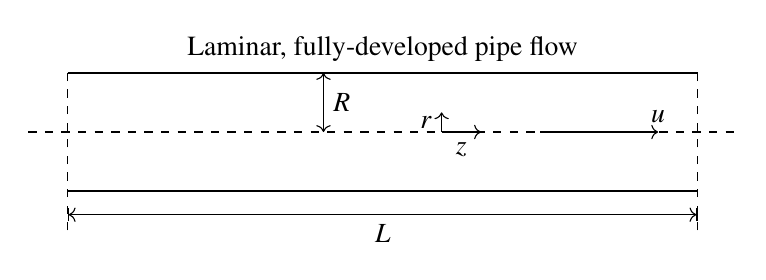
\begin{tikzpicture}
    \draw[thick] (-4,0) -- (4,0); 
    \draw[thick] (-4,1.5) -- (4,1.5);
    \draw[dashed] (-4,-0.5)--(-4,1.5);
    \draw[dashed](4,-0.5)--(4,1.5);
    \node at (0,1.8) {Laminar, fully-developed pipe flow};
    \draw[dashed] (-4.5,0.75) -- (4.5,0.75);
    \draw[->] (2,0.75) -- (3.5,0.75) node[above] {$u$};
    \draw[<->] (-0.75,0.75) -- (-0.75,1.5) node[midway, right] {$R$};
    \draw[->] (0.75,0.75) -- (0.75,1) node[midway, left] {$r$};
    \draw[|<->|] (-4,-0.3) -- (4,-0.3) node[midway, below] {$L$};
    \draw[->] (0.75,0.75) -- (1.25,0.75) node[midway, below] {$z$};
\end{tikzpicture}
  
    \end{figure}

    \item The two-dimensional velocity field $\vec{V}$ of a flow in a Cartesian coordinate system is given in dimensionless form by $$\vec{V} = (x^2-axy) \, \hat{i} + (bxy-\frac{y^2}{2}) \, \hat{j}$$
    Here, i and j are the unit vectors along the x and y directions respectively, $a$ and $b$ are independent of x,y and time. If the flow is incompressible,then the value of $(a - b)$, up to one decimal place is {\underline{\hspace{2cm}}}.

    \item For the configuration shown in the figure, oil of density $800 \, \text{kg/m}^3$ lies above water of density $1000 \, \text{kg/m}^3$. Assuming hydrostatic conditions and acceleration due to gravity $g = 10 \, \text{m/s}^2$, the length $L$ (in meters, up to one decimal place) of water in the inclined tube {\underline{\hspace{2cm}}}.
     \begin{figure}[H]
        \centering
        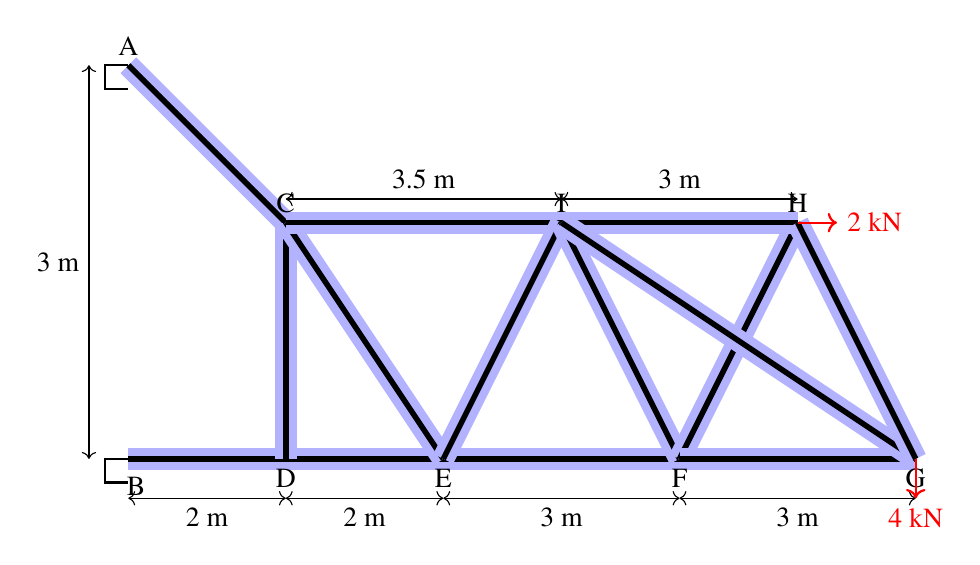
\begin{tikzpicture}
    \coordinate (A) at (0,5);
    \coordinate (B) at (0,0);
    \coordinate (C) at (2,3);
    \coordinate (D) at (2,0);
    \coordinate (E) at (4,0);
    \coordinate (I) at (5.5,3);
    \coordinate (F) at (7,0);
    \coordinate (H) at (8.5,3);
    \coordinate (G) at (10,0);
    \draw[line width=8pt, blue!30] (B) -- (D);
    \draw[line width=2pt, black] (B) -- (D);
    \draw[line width=8pt, blue!30] (D) -- (E);
    \draw[line width=2pt, black] (D) -- (E);
    \draw[line width=8pt, blue!30] (E) -- (F);
    \draw[line width=2pt, black] (E) -- (F);
    \draw[line width=8pt, blue!30] (F) -- (G);
    \draw[line width=2pt, black] (F) -- (G);
    \draw[line width=8pt, blue!30] (A) -- (C);
    \draw[line width=2pt, black] (A) -- (C);
    \draw[line width=8pt, blue!30] (C) -- (D);
    \draw[line width=2pt, black] (C) -- (D);
    \draw[line width=8pt, blue!30] (C) -- (E);
    \draw[line width=2pt, black] (C) -- (E);
    \draw[line width=8pt, blue!30] (C) -- (I);
    \draw[line width=2pt, black] (C) -- (I);
    \draw[line width=8pt, blue!30] (E) -- (I);
    \draw[line width=2pt, black] (E) -- (I);
    \draw[line width=8pt, blue!30] (I) -- (F);
    \draw[line width=2pt, black] (I) -- (F);
    \draw[line width=8pt, blue!30] (F) -- (H);
    \draw[line width=2pt, black] (F) -- (H);
    \draw[line width=8pt, blue!30] (G) -- (F);
    \draw[line width=2pt, black] (G) -- (F);
    \draw[line width=8pt, blue!30] (H) -- (I);
    \draw[line width=2pt, black] (H) -- (I);
    \draw[line width=8pt, blue!30] (I) -- (G);
    \draw[line width=2pt, black] (I) -- (G);
    \draw[line width=8pt, blue!30] (H) -- (G);
    \draw[line width=2pt, black] (H) -- (G);
    \draw[thick] (A) -- ++(-0.3,0) -- ++(0,-0.3) -- ++(0.3,0);
    \draw[thick] (B) -- ++(-0.3,0) -- ++(0,-0.3) -- ++(0.3,0);
    \node[above] at (A) {A};
    \node[below] at (0.1,-0.1) {B};
    \node[above] at (C) {C};
    \node[below] at (D) {D};
    \node[below] at (E) {E};
    \node[above] at (I) {I};
    \node[below] at (F) {F};
    \node[above] at (H) {H};
    \node[below] at (G) {G};
    \draw[<->, thin] (B)++(0,-0.5) -- node[below] {2 m} ++(2,0);
    \draw[<->, thin] (D)++(0,-0.5) -- node[below] {2 m} ++(2,0);
    \draw[<->, thin] (E)++(0,-0.5) -- node[below] {3 m} ++(3,0);
    \draw[<->, thin] (F)++(0,-0.5) -- node[below] {3 m} ++(3,0);
    \draw[<->, thin] (A)++(-0.5,0) -- node[left] {3 m} ++(0,-5);
    \draw[<->, thin] (C)++(0,0.3) -- node[above] {3.5 m} ++(3.5,0);
    \draw[<->, thin] (I)++(0,0.3) -- node[above] {3 m} ++(3,0);
    \draw[red, thick, ->] (H) -- ++(0.5,0) node[right] {2 kN};
    \draw[red, thick, ->] (G) -- ++(0,-0.5) node[below] {4 kN};
\end{tikzpicture}

  
    \end{figure}

    \item A two-dimensional Eulerian velocity field is given (in m/s) by $\vec{V} = \left( \sqrt{5} x \right) \, \hat{i} - \left( \sqrt{12} y \right) \, \hat{j}$, where $x$ and $y$ are the coordinates (in meters) in a Cartesian coordinate system.The magnitude of the acceleration (in $\text{m/s}^2$, up to one decimal place) of a fluid particle at $x = 1 \, \text{m}$ and $y = -1 \, \text{m}$ is {\underline{\hspace{2cm}}}.
   

    \item A large pump is to deliver oil at an average velocity $V$ of  1.5$m/s$. The pump has an impeller diameter $(D)$ of 40cm and the pressure rise across the pump is $400{kPa}$. To design this pump, a lab-scale model pump with an impeller diameter of $4{cm}$ is to be used with water as the fluid. The viscosity $(\mu)$ of the oil is 100 times that of water, and the densities $(\rho)$ of oil and water are identical. A complete geometric similarity is maintained between the model and prototype. If the pressure rise is a function only of $V$, $D$, $\rho$, and $\mu$, the pressure rise (in kPa, up to one decimal place) across the model pump is {\underline{\hspace{2cm}}}.

    \item Water (density = $1000  \text{kg/m}^3$) enters steadily into a horizontal pipe bend, which is part of a larger piping system, as shown in the figure. The volumetric flow rate of water is $0.1 \, \text{m}^3/\text{s}$. The gage pressure at the inlet is $500\text{kPa}$, while the exit is open to the atmosphere. The $x$-component of the force on the support $F_x$.The absolute value of $F_x$(in kN, up to one decimal place) is {\underline{\hspace{2cm}}}.
    \begin{figure}[H]
        \centering
        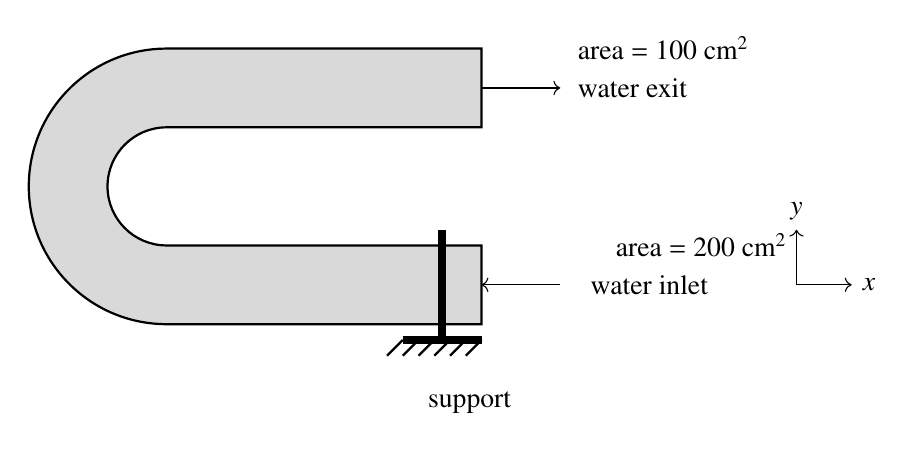
\begin{tikzpicture}
    \draw[thick, fill=gray!30] (0,0.5) -- (4,0.5) -- (4,1.5) -- (0,1.5) arc[start angle=270, end angle=90, radius=0.75] -- (0,3) -- (4,3) -- (4,4) -- (0,4) arc[start angle=90, end angle=270, radius=1.75]--(0,0.5) -- cycle;
    \draw[<-] (4,1) -- (5,1);
    \draw[->] (4,3.5) -- (5,3.5); 
    \node at (4.5,-0.5) [left] {support};
    \draw[line width=1mm](3.5,0.3)--(3.5,1.7);
    \draw[line width=1mm](3,0.3)--(4,0.3);
    \draw[thick](3,0.3)--(2.8,0.1);
    \draw[thick](3.2,0.3)--(3,0.1);
    \draw[thick](3.4,0.3)--(3.2,0.1);
    \draw[thick](3.6,0.3)--(3.4,0.1);
    \draw[thick](3.8,0.3)--(3.6,0.1);
    \draw[thick](4,0.3)--(3.8,0.1);
    \node at (7,1) [left] {water inlet};
    \node at (8,1.5) [left] {area = 200 cm$^2$};
    \node at (5.1,3.5) [right] {water exit};
    \node at (5.1,4) [right] {area = 100 cm$^2$};
    \draw[->] (8,1) -- ++(0.7,0) node[right] {$x$};
    \draw[->] (8,1) -- ++(0,0.7) node[above] {$y$};
\end{tikzpicture}

  
    \end{figure}

\end{enumerate}

\end{document}


